% Created 2026-09-11 sex 14:50
% Intended LaTeX compiler: pdflatex
\documentclass[11pt]{article}
\usepackage[utf8]{inputenc}
\usepackage[T1]{fontenc}
\usepackage{graphicx}
\usepackage{longtable}
\usepackage{wrapfig}
\usepackage{rotating}
\usepackage[normalem]{ulem}
\usepackage{amsmath}
\usepackage{amssymb}
\usepackage{capt-of}
\usepackage{hyperref}
\author{wgn}
\date{\today}
\title{Apresentação da Ferramenta Gepis Dados Abertos}
\hypersetup{
 pdfauthor={wgn},
 pdftitle={Apresentação da Ferramenta Gepis Dados Abertos},
 pdfkeywords={},
 pdfsubject={},
 pdfcreator={Emacs 30.2 (Org mode 9.7.11)}, 
 pdflang={English}}
\begin{document}

\maketitle
\tableofcontents

Objetivando apoiar a cultura e reúso de dados abertos, o grupo de pesquisa GEPIS apresenta sua ferramenta de exploração e reúso de dados abertos.

A ferramenta foi está sendo desenvolvida com ajuda do Gemini e do Claude, é de código livre (licença GNU) e está hospedada em \url{https://github.com/grupo-de-pesquisa-gepis/gepisopendata}

A apresentação será totalmente de forma prática e conceitos ou informações específicas são apresentadas oportunamente nos diversos momentos da prática.
\section{Instalação}
\label{sec:org3a78799}
\subsection{Fazendo do download}
\label{sec:org3be4edd}
\begin{itemize}
\item entrar no \href{https://github.com/grupo-de-pesquisa-gepis/gepisopendata/releases}{link de releases }
\item baixar a última versão

\begin{center}
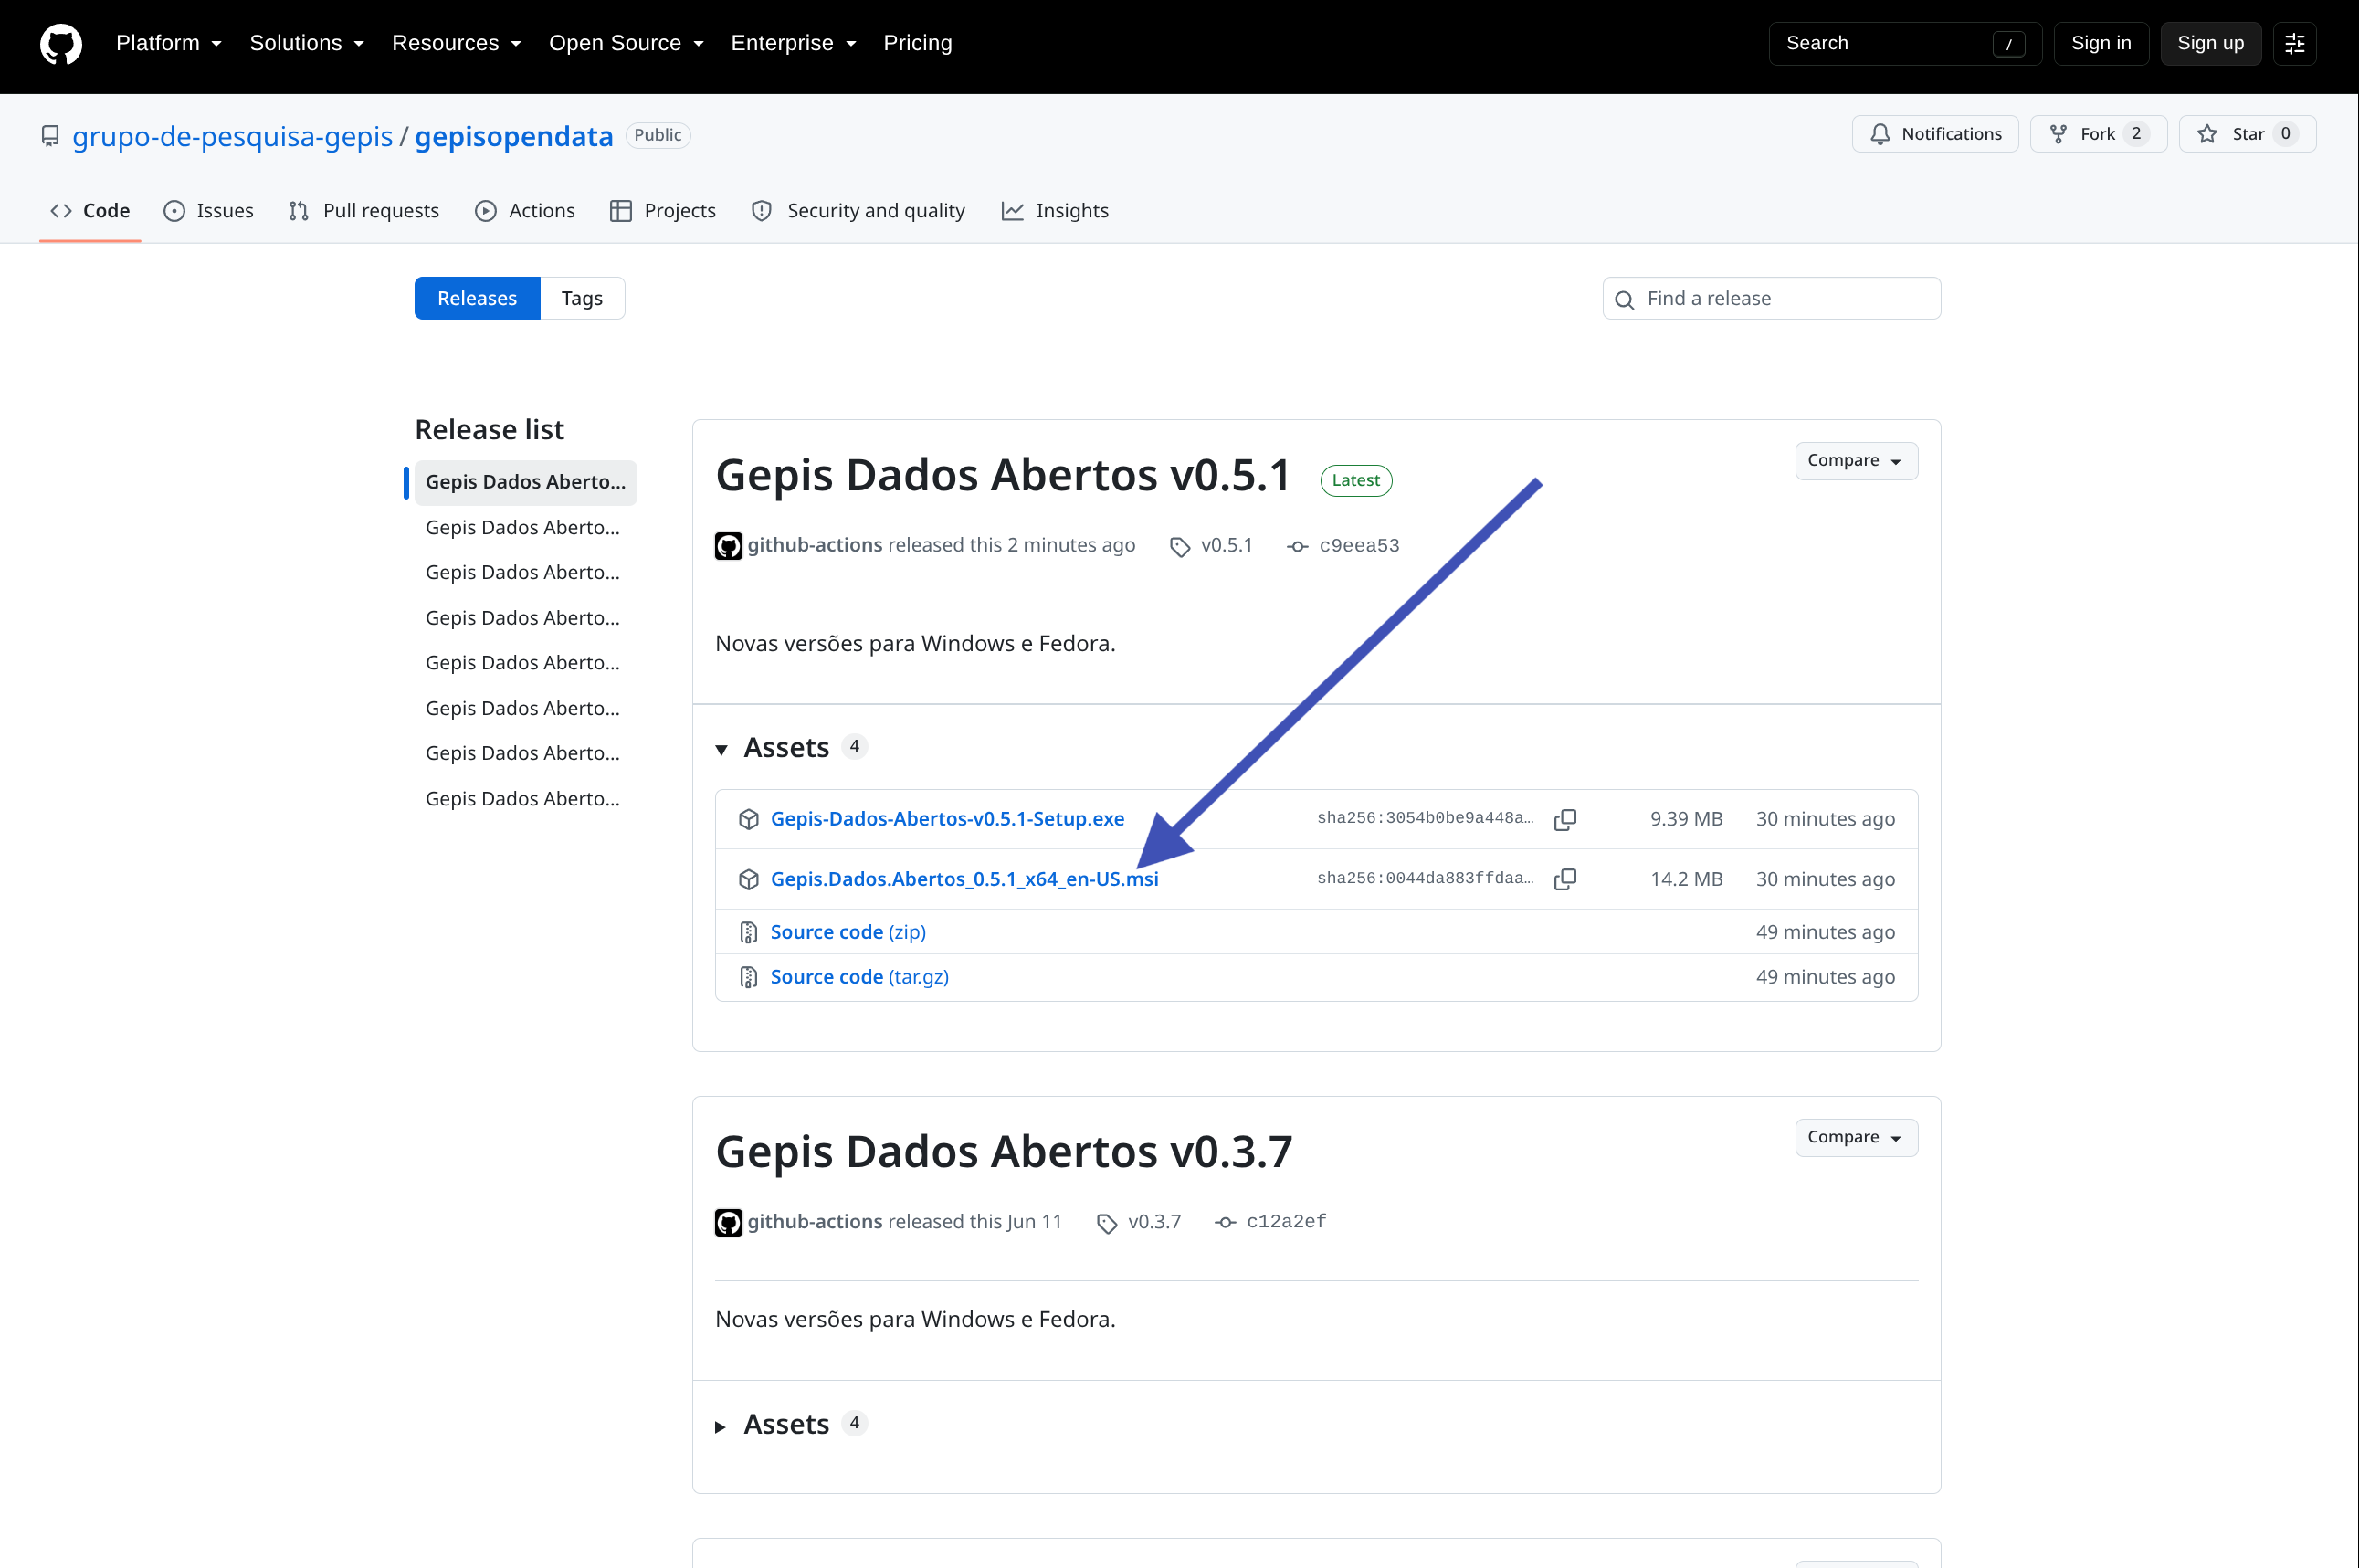
\includegraphics[width=.9\linewidth]{./imgs-apresentacao/img1.png}
\end{center}
\end{itemize}
\section{Configuração}
\label{sec:org2fc5a22}

\section{Obtendo os microdados}
\label{sec:orgde63422}

\section{Aspectos Técnicos}
\label{sec:org5bfae54}
\end{document}
